\documentclass[twoside,11pt, letter]{article}

\setlength{\textheight}{23cm}
\setlength{\textwidth}{17cm}
\setlength{\topmargin}{-0.2cm}
%\setlength{\bottommargin}{1.0cm}
\setlength{\oddsidemargin}{-0.2cm}
\setlength{\evensidemargin}{-0.2cm}
%----------------------------
%Remove a lot of white space:
%\setlength{\textfloatsep}{1cm}
\setlength{\textfloatsep}{1ex plus 2.0pt minus 2.0pt}
\setlength{\floatsep}{1ex plus 2.0pt minus 2.0pt}
\setlength{\intextsep}{1ex plus 2.0pt minus 2.0pt}
\setlength{\abovecaptionskip}{1ex}
\setlength{\belowcaptionskip}{0pt}

%\include{typelayout}
%----------------------------

\headsep = 8pt
\usepackage{graphicx}
\graphicspath{{./}{figures/}}
\usepackage{color}
\usepackage{subfigure}
\usepackage{amsmath,amsfonts}
\usepackage{mathptmx}
\usepackage{bm} 
\usepackage{enumerate}
%\usepackage{floatflt}
\usepackage{wrapfig} %similar to floatflt, but couldn't find reduction of
                     %horiz. spacing for floatflt.
\usepackage{longtable}

% By default, LaTeX doesn't like to fill more than 0.7 of a text page with tables
% and graphics, nor does it like too many figures per page. 
\renewcommand{\floatpagefraction}{0.9}
\renewcommand{\topfraction}{0.9}
\renewcommand{\bottomfraction}{0.9}
\renewcommand{\textfraction}{0.1}
\newcommand{\1}[1]{\, \mathrm{#1}} % unit(y ;-)

\setcounter{totalnumber}{50}
\setcounter{topnumber}{50}
\setcounter{bottomnumber}{50}

\setlength{\columnsep}{3ex}

\usepackage{fancyhdr}
%\pagestyle{fancy}
\lhead[\fancyplain{}{}]{\fancyplain{}{\slshape \rightmark}}
\rhead[\fancyplain{}{\slshape \nouppercase{\leftmark}}]{\fancyplain{}{}}
\cfoot{\thepage}
%\renewcommand{\headrulewidth}{0.4pt}

%\setlength{\headheight}{14pt}

%\bibliographystyle{melga_unsrt}

\begin{document}

%\pagestyle{fancy}
%\setcounter{page}{1}
\section{Introduction}
My first thought for this challenge was not to use some kind of machine learning algorithm, so I'll present two solutions.  
In both cases, I assume that the most useful questions are those which were answered correctly by about 63\% of students from the previous year.  
My reasoning is simply that a question which everyone gets right or wrong is not useful, as it does not add information about how the students compare to one another.
I chose 63\% (rather than 50\%) as a baseline because that turned out to be the mean number of correct responses for all questions.

\section{SVM method}
The first solution I wanted to present uses NumPy's SVM functionality to classify `good' and `bad' questions.
I chose two features to describe the data: the number of responses for each question last year, and the fraction of correct responses to that question.
I then trained the SVM using simulated data, drawn by hand.
The goal again is to define `good' questions as those which were answered correctly about 60\% of the time using the historical data.
The number of responses per question was used to `tighten' the definition of the allowed deviation from the mean, similar in principle to the use of the variance in Solution 1.

After training, the SVM was used to predict `good' and `bad' questions by running over the historical data from last year's exam.
For the choice of questions, the result of this calculation would be viewed as a binary output: `good' questions would be randomly sampled to make this year's test, `bad' questions would be ignored.
I include plots of the test data and final output in Figure 1.
The code for this calculation outputs a list of good questions as well as a sample test for this year (implimented by drawing randomly from the list of approved questions).
Long term, I believe this method would preferable to the one I present next, primarily because it is much more likely to benefit from additional information

\begin{figure}
\begin{center}
\subfigure[Training data]{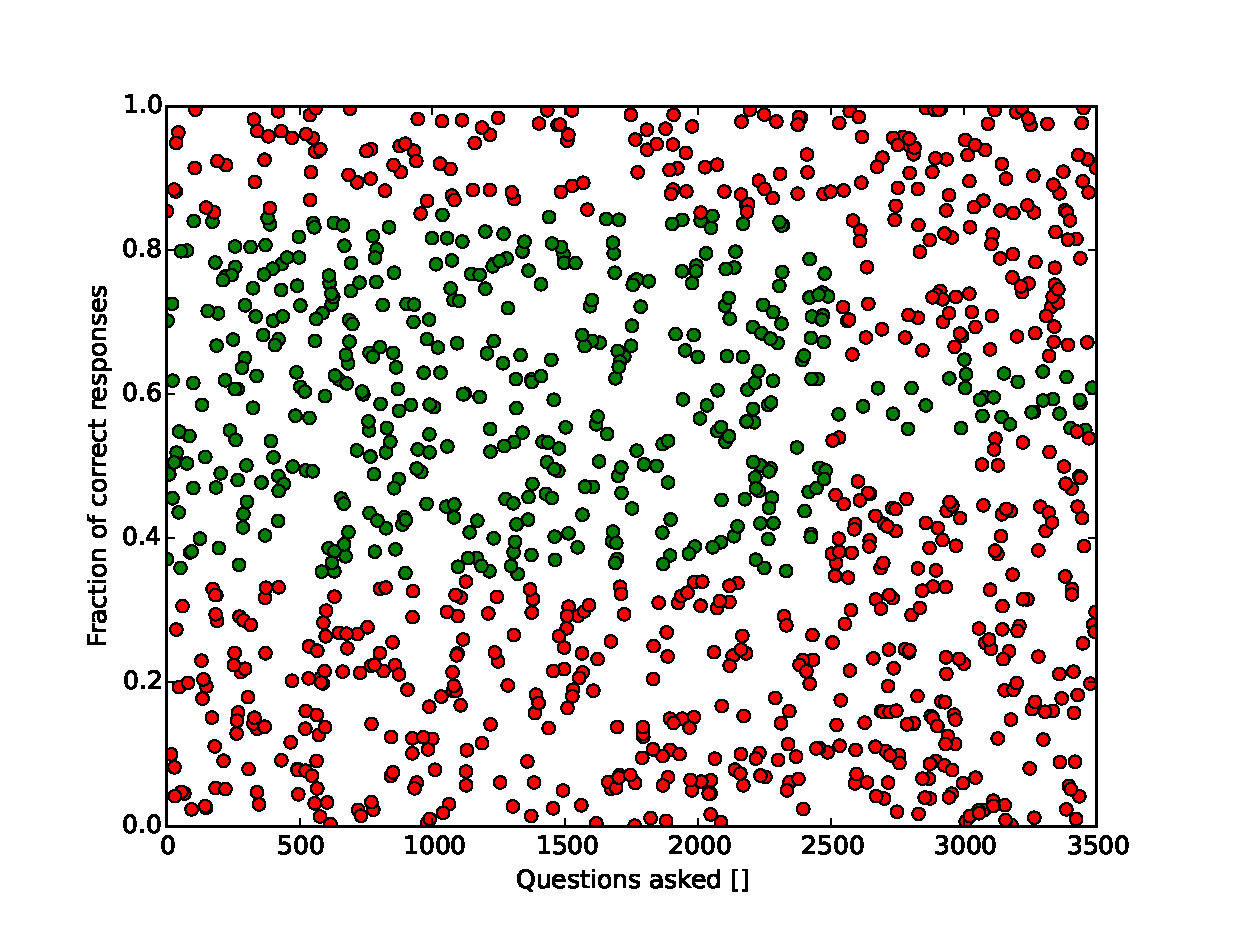
\includegraphics[scale=0.4]{plots/test_data.eps}}
\subfigure[Old test scores]{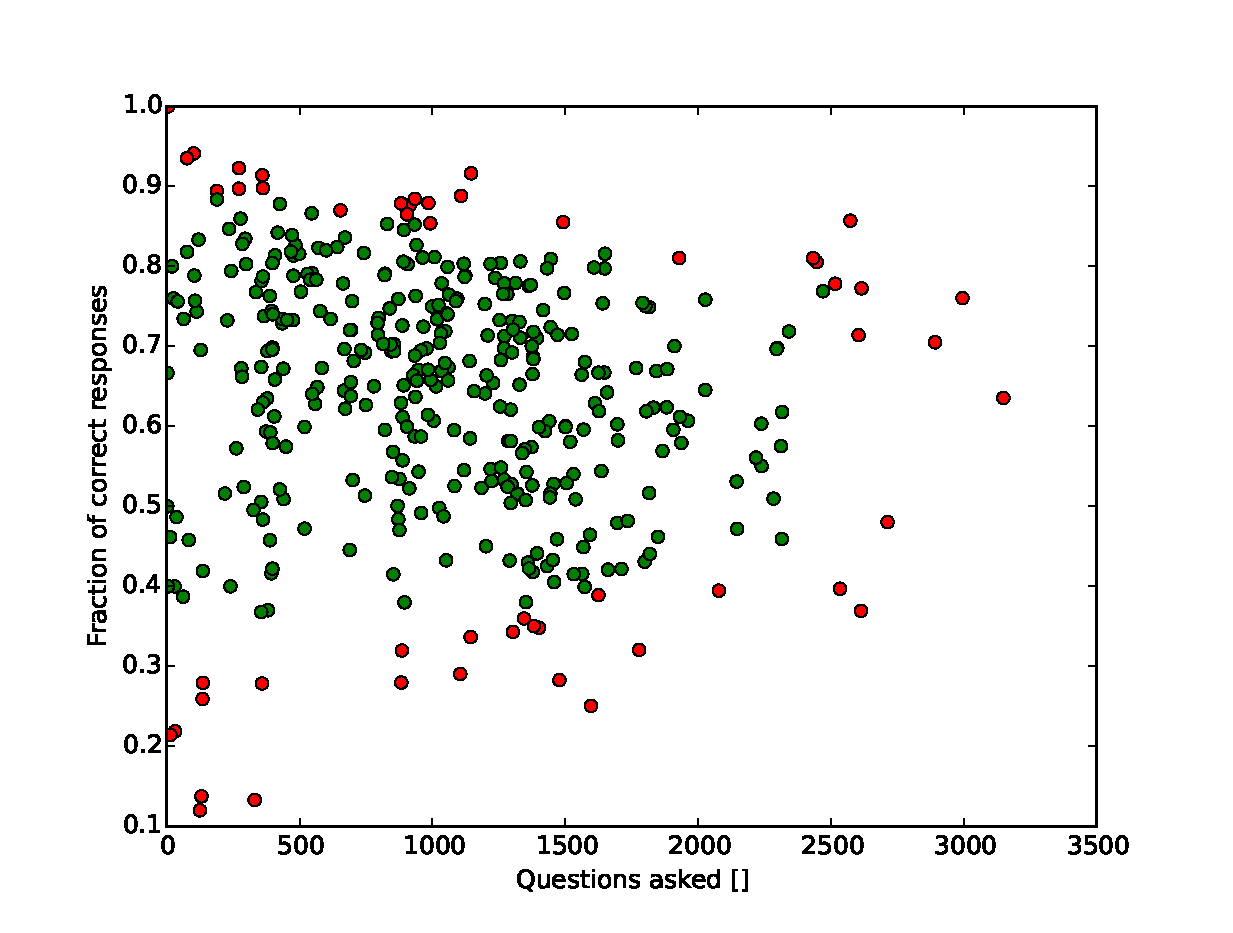
\includegraphics[scale=0.4]{plots/frac_vs_num_scatter.eps}}
\caption{Simulated data used to train the SVM (left) and historical test score data (right).  In both cases, red dots are considered `bad' and green dots are considered `good.'}
\end{center}
\end{figure}

\newpage

\section{Weight method}
The next solution to present is actually the first one that came to my mind when reading the question.
Rather than using machine learning, I simply plotted the distribution of the fraction of correct responses for each question and used this to define a set of weights that can be used to `steer' the sampling process.
The goal is to increase the probability of sampling good questions but still cover the entire curriculum (in principle).

Since the distribution of the fraction of correct responses appears approximately Gaussian, I calculated the difference between each question's fraction of correct answers and the mean of the whole distribution, normalized to the statistical uncertainty on the fraction.
Note that including the statistical uncertainty may not be the best choice, if the goal is to be as aggressive as possible in removing bad questions.
I assume, basically, that the questions were well-conceived, and that we should not penalize a particular question simply because not many students responded to it.
If you trust the content of the questions less, it could be worth only accepting a question if you are confident it is good (i.e. ignoring the statistical uncertainty).

I then use this normalized deviation to define a weight for each question according to:

\begin{equation*}
\displaystyle w_i = e^{-\frac{x_i - \mu}{\sigma_i}}
\end{equation*}

\noindent where $w_i$ is the weight, $x_i$ is the fraction of correct responses, $\mu$ is the average fraction for all questions, and $\sigma_i$ is the statistical uncertainty on the fraction.
Figure 2 shows the distribution of these weights.
The weight is then used when selecting questions for this year's test: instead of drawing questions at random, they are drawn with a frequency equal to the calculated weight.
Questions with a higher weight will be chosen more frequently, so the most frequent choices will have approximately the mean number of right answers from the previous year.

The choice of how to define the weights is an open one, but I chose an exponential primarily to give the highest weight to those questions with nearest the mean number of correct responses.
Before being used to sample test questions, the weights are normalized to their total sum, meaning that only the relative magnitude of each weight is important.
The code for this portion of the calculation outputs a list of weights and a sample test generated using this method.
As mentioned above, this method wouldn't scale as nicely when new variables are added, but given the relatively simple nature of the data set, I thought this method was worth pursuing.

\begin{figure}
\begin{center}
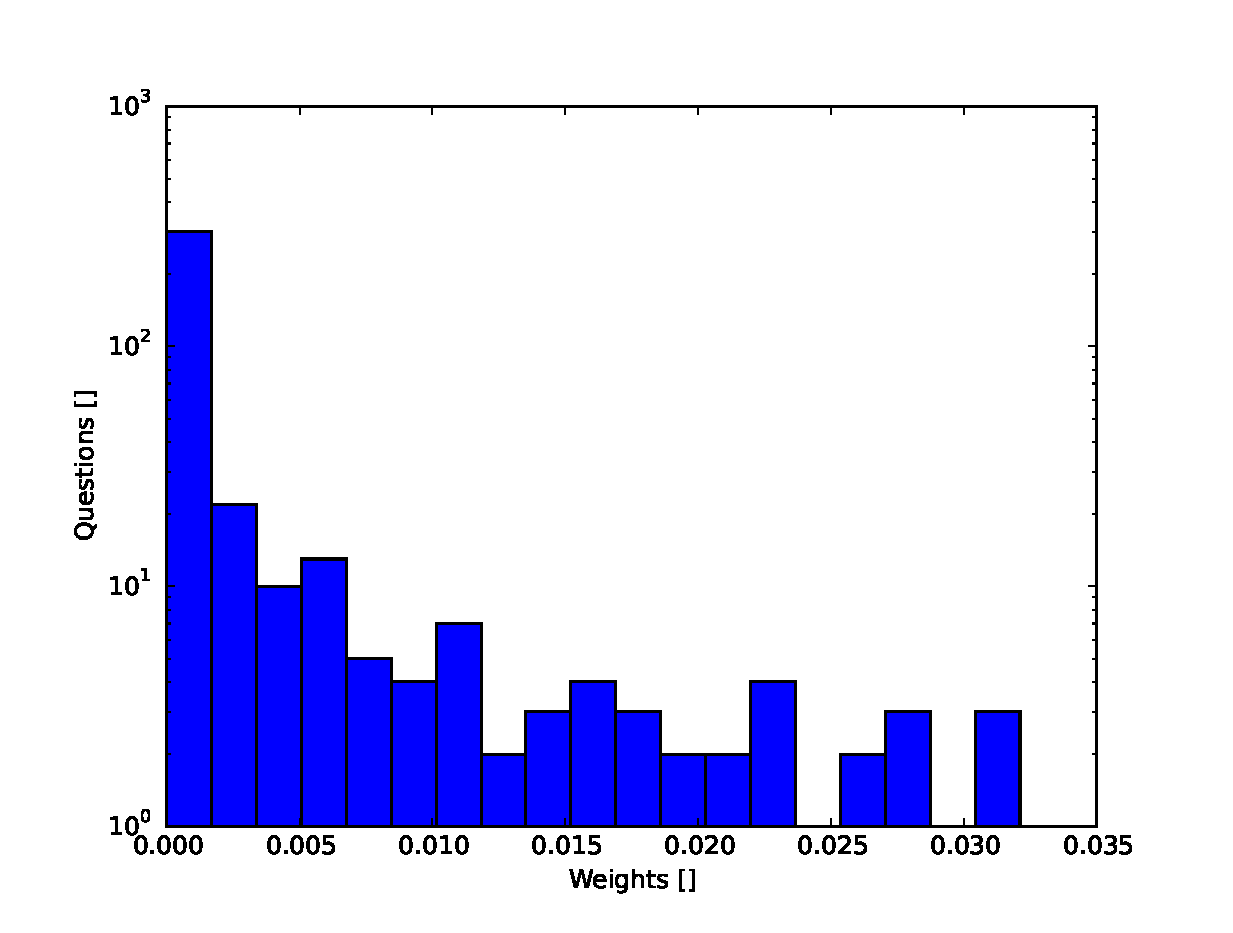
\includegraphics[scale=0.4]{plots/weights.eps}
\caption{Absolute weight for each question (i.e. prior to normalization).  Weights are based on deviation from the mean of the fraction of correct responses received for each question in last year's data.}
\end{center}
\end{figure}

\end{document}
